\begin{figure}[H]
    \centering
    \definecolor{curveblue}{RGB}{35,105,180}
    \definecolor{accentred}{RGB}{185,45,45}
    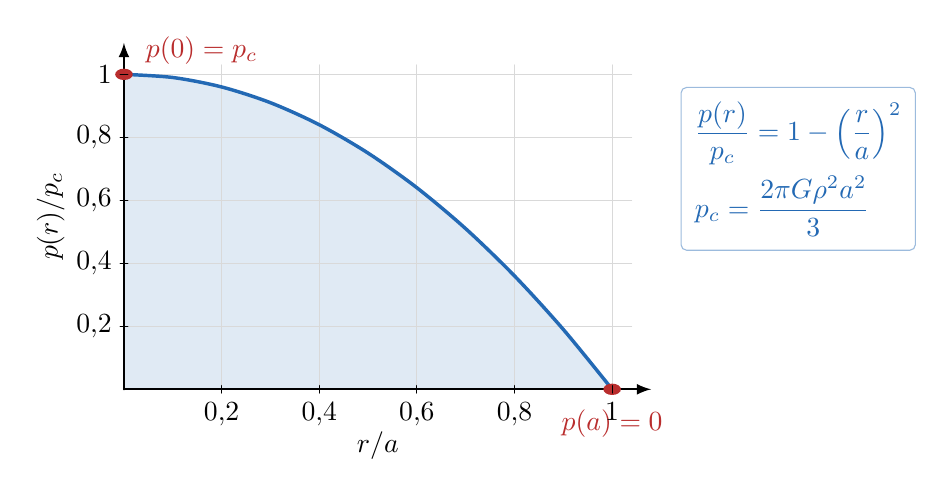
\begin{tikzpicture}[x=6.2cm,y=4.0cm,line cap=round,line join=round]
        % Área bajo el perfil
        \fill[curveblue!14]
            (0,0) --
            plot[smooth] coordinates {
                (0,1) (0.1,0.99) (0.2,0.96) (0.3,0.91)
                (0.4,0.84) (0.5,0.75) (0.6,0.64) (0.7,0.51)
                (0.8,0.36) (0.9,0.19) (1,0)
            } -- cycle;

        % Retícula
        \foreach \x in {0.2,0.4,0.6,0.8,1.0} {
            \draw[black!15] (\x,0) -- (\x,1.03);
        }
        \foreach \y in {0.2,0.4,0.6,0.8,1.0} {
            \draw[black!15] (0,\y) -- (1.04,\y);
        }

        % Ejes y curva
        \draw[-latex,line width=0.8pt] (0,0) -- (1.08,0);
        \draw[-latex,line width=0.8pt] (0,0) -- (0,1.10);
        \draw[curveblue,line width=1.25pt,smooth]
            plot coordinates {
                (0,1) (0.1,0.99) (0.2,0.96) (0.3,0.91)
                (0.4,0.84) (0.5,0.75) (0.6,0.64) (0.7,0.51)
                (0.8,0.36) (0.9,0.19) (1,0)
            };

        % Puntos característicos
        \fill[accentred] (0,1) circle (0.018);
        \node[accentred,above right] at (0.025,1.00)
            {$p(0)=p_c$};
        \fill[accentred] (1,0) circle (0.018);
        \node[accentred,below] at (1,-0.035)
            {$p(a)=0$};

        % Títulos de los ejes, separados de las marcas numéricas
        \node at (0.52,-0.18) {$r/a$};
        \node[rotate=90] at (-0.15,0.55) {$p(r)/p_c$};

        % Expresión del perfil en una zona independiente del gráfico
        \node[
            curveblue,
            draw=curveblue!45,
            fill=white,
            rounded corners=2pt,
            inner sep=5pt,
            align=left,
            anchor=west
        ] at (1.14,0.70)
            {$\displaystyle \frac{p(r)}{p_c}
              =1-\left(\frac{r}{a}\right)^2$\\[3pt]
             $\displaystyle p_c=\frac{2\pi G\rho^2a^2}{3}$};

        \foreach \x/\lab in {0.2/{0{,}2},0.4/{0{,}4},0.6/{0{,}6},0.8/{0{,}8},1/{1}} {
            \draw (\x,0.012) -- (\x,-0.012);
            \node[below] at (\x,-0.01) {$\lab$};
        }
        \foreach \y/\lab in {0.2/{0{,}2},0.4/{0{,}4},0.6/{0{,}6},0.8/{0{,}8},1/{1}} {
            \draw (0.008,\y) -- (-0.008,\y);
            \node[left] at (-0.005,\y) {$\lab$};
        }
    \end{tikzpicture}
    \caption{Perfil normalizado de presión dentro de un planeta de densidad constante.}
\end{figure}
